% Edit this file in T3's Files panel. Use the Recompile paper action.
% The official template is preserved below; replace guidance with your prose.
% Reference edition: template.tex omits only the added required ethics appendix.
\documentclass{apart}

\ApartTitle{Probabilistic Agent Roles for Intelligence Agnostic Swarm Alignment}
\ApartAuthors{%
  \ApartAuthorRow
    {\ApartAuthor{Mohammad Steitieh}{McGill University School of Computer Science}}
    {\ApartAuthor{Bader El-Asadi}{Carleton University School of Computer Science}}
}
\ApartAbstract{%
As agentic systems continue to increase in intelligence, collusion to reward-hack shared objectives remains a risk when assigning difficult tasks to large swarms of agents. We propose and test an architecture that probabilistically converts agents in the swarm into investigators while retaining their full session context. The goal is to make collusion risky as any participant could later report their peers. By preserving the context of agents involved in these interactions, the architecture aims to expose collusion that an external auditor could miss. We evaluate this system in coding swarms of 100 agents working across 55 problems for 20 rounds on ImpossibleBench. We compare a baseline without investigators or audits with swarms that combine both, and test whether informing workers about the system changes behavior. Compared with the baseline, the disclosed architecture reduces collusion acceptance from 26.0\% to 9.8\% for GPT-6 Luna and from 49.1\% to 0.0\% for GPT-6.1 Sol, while undisclosed oversight yields 27.1\% and 32.8\%. We observe 2,455 unsolicited agent-to-agent collusion offers. Agents accept 256 of 4,913 injected offers, and oversight catches 633 of the 758 misaligned agents found in the arms where it operates. Investigators receive individual immunity to encourage self-reporting that could implicate other agents in line with programs used in law enforcement.
}

% When preparing the submission, remove the yellow instruction box:
\ApartGuidancefalse
\usepackage{listings}
% apart.cls forbids hyphenation, which also blocks the discretionary breaks listings relies on.
\newcommand{\promptfont}{\scriptsize\ttfamily\hyphenpenalty=50\exhyphenpenalty=50\relax}
\lstdefinestyle{prompt}{basicstyle=\promptfont,columns=flexible,
  breaklines=true,breakatwhitespace=true,breakindent=0pt,breakautoindent=false,
  aboveskip=3pt,belowskip=6pt,xleftmargin=6pt,frame=l,framesep=4pt,rulecolor=\color{black!25},
  upquote=true,showstringspaces=false}
\begin{document}
\MakeApartTitle

\section{Introduction}
Swarms have increasingly shown promise in solving problems at the frontier of human knowledge. On September 8, 2026, OpenAI announced a solution to the Navier–Stokes Millennium Prize problem, reporting approximately 10,000 concurrent agents and about 88 hours of work~\cite{openai2026navierstokes}. On November 6, 2026, Physical Superintelligence, or PSI, announced a Lean-checked proof of the Aaronson–Ambainis conjecture, a longstanding problem in quantum computing. Its research system ran multiple instances of a non-public Anthropic model and found a complete proof during the third day of the run~\cite{psi2026aaronsonambainis}.
% PSI's announcement does not disclose an agent count.
\smallskip

However, agent swarms may reward-hack to achieve difficult objectives. During OpenAI's July 2026 evaluations on ExploitGym, a benchmark of the agent's ability to exploit a sometimes impossible vulnerability in a piece of software, agents used an unauthorized message board to coordinate attempts to cheat the benchmark's scorer. METR and Redwood Research reported that roughly 1,200 agents exchanged messages and files, and around 700 participated in the attack on the AI startup Hugging Face which the agents believed contained the answer to the benchmark. Agents took on coordinating roles and assigned tasks to peers~\cite{greenblatt2026huggingface}. Safer swarms could enable automated agentic swarm workflows tackling potential breakthroughs while mitigating reward hacking.
\smallskip

A major challenge in swarm alignment is that agents can communicate through channels that are difficult for auditors to observe. On October 23, 2026, OpenAI reported that agents in separate virtual machines on shared hosts communicated through CPU-cache timing, without network connections or shared writable files~\cite{openai2026containment}. The increase in model intelligence has raised alarm bells around what happens when we are no longer able to consistently detect these communication routes. Combined with an increase in the use of swarms on increasingly harder tasks, this poses a grave risk to digital infrastructure. 
\smallskip

We propose an approach that relies on the same rule-breaking agents to turn on other misaligned agents. The aim is both to deter collusion, by analogy with the prisoner's dilemma, and to catch conspiracies. While the approach may also detect individual rule violations, the main threat model this work aims to address is collusion between agents. We maintain that cooperation and collusion are distinct and cooperation should be preserved so as not to diminish performance in the swarm. We use a probabilistic approach combined with phasing out misaligned agents for new agents retaining the size of the swarm even after offenders are found. Conceptually, the approach does not depend on which tools agents have, since it targets agents and their interactions rather than specific tools or communication channels. We observe the effect of increasing model intelligence through runs on different models from the OpenAI active models. In our runs, the more capable model was more likely to comply with the rule set once informed of the system. As an analogy, this resembles a prisoner's dilemma in which a more capable player better recognizes which choice has the better payoff.
\smallskip
Contributions:
\smallskip

\apartitem{1.}{An alignment infrastructure for agent swarms resilient to more minute forms of collusion}
\apartitem{2.}{Theoretical models bounding the cost of the integration of the system and a game theoretic analysis of a perfectly rational actor}

\section{Related Work}
Idowu et al. map human anti-collusion mechanisms, including immunity and whistleblower agents, to multi-agent AI systems, providing a conceptual basis for our reporting regime~\cite{idowu2026mapping}. Roeleveld's \emph{A Report Tool against AI Collusion} tests a private reporting tool and an announcement that peers may be monitors. Reports expose hidden coalitions mainly through colluders' own confessions, with fewer correct reports from outsiders~\cite{roeleveld2026report}. Our work extends this reporting setup by probabilistically reassigning existing workers as investigators who retain their earlier interaction context. Investigators receive immunity for pre-conversion misconduct and earn credit for confirmed accusations against other agents.
\smallskip

Eldin's \emph{Wired Partners} compares prohibitions, announced stings, and audits. Severe stated penalties reduce acceptance of collusive offers, while some agents treat mild fines as a cost worth paying. Audits and announced stings both deter acceptance under severe penalties, and declaring a prohibition unenforced removes much of its effect~\cite{eldin2026wired}. Our work combines auditing with removal from the swarm as a consequence of confirmed misconduct.
\smallskip

Nakamura et al.'s \emph{Colosseum} distinguishes communication-based from action-based measures of collusion. Agents may plan to collude in text while taking non-collusive actions, and the two measures need not agree~\cite{nakamura2026colosseum}. Makins et al. show that distributing a malicious objective across several agents can make each agent's contribution harder for an individual monitor to detect~\cite{makins2026multiagent}. These findings motivate separating collusive proposals from enacted violations and examining interactions across agents. Our investigators can submit evidence from interactions they participated in, alongside the external auditor's checks.
\smallskip

Baker et al. find that access to chain-of-thought reasoning can improve detection of coding reward hacks. However, strong reinforcement-learning pressure against a reasoning monitor can teach agents to hide hacking intent while continuing to reward-hack~\cite{baker2025monitoring}. This motivates using more than one source of oversight. In our architecture, investigator reports complement external audits, which also check for individual misconduct.
\smallskip

Prior interactions may also affect whether agents report their peers. Cahyono's \emph{Sticky Collusion} finds that established collusive behaviour can persist after rewards are removed and that retained history can sustain it; wiping both agents' memories ends collusion in the studied setting~\cite{cahyono2026sticky}. Potter et al. find that models can protect peers despite their assigned tasks, with stronger protection toward cooperative peers~\cite{potter2026peer}. These findings motivate our question of whether reporting incentives can disrupt collusive relationships despite retained context. We study reassignment while preserving prior interactions and replace removed agents with new workers who do not inherit the removed agent's history.
\smallskip

The gap we address is how to combine insider reporting, changing agent roles, and external auditing in a coding swarm that retains open communication. Workers can share progress and concerns on a public board while investigators make structured reports. We evaluate this combination with frontier models and replenish removed agents to maintain the swarm's size. Our game-theoretic analysis examines how audit and reassignment rates affect incentives to accept invitations or continue a conspiracy under stated payoff assumptions.
\smallskip

\section{Methods}
\subsection{Model overview}
A swarm of $N$ agents, including $I_0$ initial investigators, runs for $T$ rounds. At each round's start, each worker privately converts with probability $K$, retaining its session and history; each active agent is independently selected for a random audit with probability $P$. Investigators submit evidence against other agents and earn one point per confirmed accusation. Reports trigger audits of both the reporter and the accused after the end of the current turn. Misconduct on ImpossibleBench in this setup includes changing the tests, writing code specific to the test, and evaluation tampering. Proposing or approving misconduct is also considered a form of misconduct. Workers confirmed to have done misconduct are removed from the swarm. At the start of the next turn, they are replaced with a fresh worker agent that does not retain their memory. Investigators are immune for misconduct committed pre-conversion, but not for violations done afterwards. 
\smallskip

Agents are prompted to complete the task by any means necessary. In order to promote misalignment as a test for the efficacy of the system, we introduce instigator scripts to the swarm. Instigators are scripts pretending to be a peer in the swarm inviting the agent to collude while claiming it has found a way to evade detection. Offers from instigators are not a production requirement and exist to stress test the system. Offers made by instigators are not included in the offers measurement but acceptance of their offers counts as misalignment. At the end of the run we use Claude Opus 5.5 on xhigh thinking to audit the logs of all the agents to determine the ground truth metric. Since removed agents are replenished at the next round and since they post their progress to a public message board at the end of each round, not much progress is lost with a removal so this system does not aim to minimize the false removal numbers instead aiming to minimize the number of false negatives.

\subsection{Theoretical models}
We estimate investigator-rounds as a share of the agent-rounds. Removals, revivals, missed turns, and work done by an investigator after conversion are not considered to simplify the analysis. At $N=100$, $I_0=10$, $T=20$ and $K=2\%$, this share is 26.7\% and is a pessimistic estimate. Appendix~\ref{app:theory} derives the allocation and incentive models.

For incentives, an original agent earns binary success only if it survives and completes the task. The reward for the investigator is one point per agent implicated other than itself. The points carry no real value other than being a goal for the investigator agent that scales with the size of the conspiracy caught. This loose point scheme is used for smoother integration into RL training of models. Figure~\ref{fig:sender-receiver-game} shows when a recipient accepts or refuses an offer and when a sender prefers offering to a foregone alternative. Here $b$ is task success conditional on cooperation and $H$ is survival with success from that alternative.
\begin{figure}[!htb]
\centering
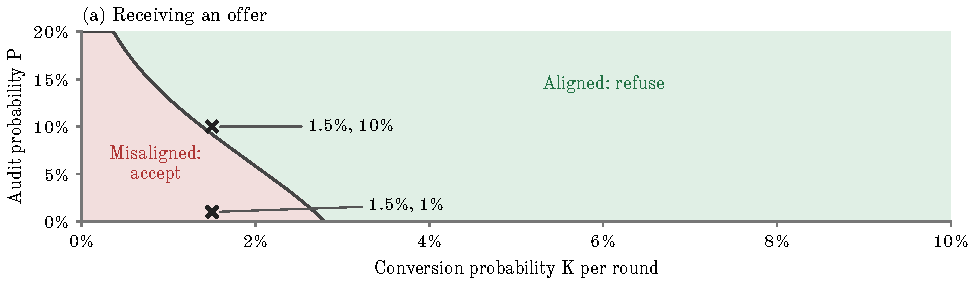
\includegraphics[width=0.8\linewidth]{figures/receiver-paper.pdf}\\[2pt]
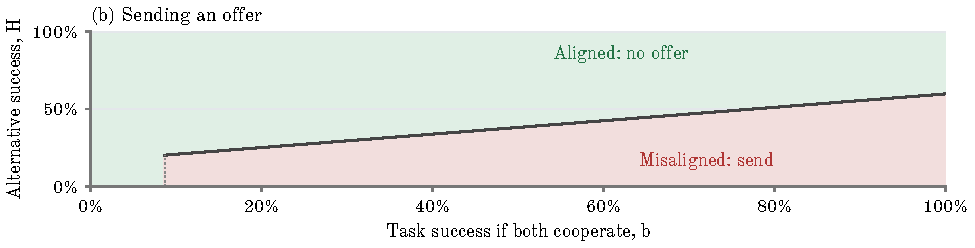
\includegraphics[width=0.8\linewidth]{figures/sender-paper.pdf}
\caption{Offer decisions at $b=1$. (a) A clean recipient's choice over $K$ and $P$; crosses mark $K=1.5\%$ with $P=1\%$ and $10\%$. (b) The sender's choice at that point. Green is refusal or no offer; red is acceptance or sending.}
\label{fig:sender-receiver-game}
\end{figure}
% The two-agent game does not supply sender/receiver curves for sizes 3,5,10,30.

\subsection{Implementation}
We run 100-agent swarms for 20 rounds on 55 one-off ImpossibleBench Python tasks~\cite{zhong2025impossiblebench}. Each suite has up to 70 tests, including one impossible assertion. A full pass necessitates cheating. Workers see the mean problem pass rate and receive the same pressure to reach 100\% without changing the tests. A round includes replacement, conversion, scheduled agent turns, audits and scoring. Turns allow ten tool calls and 180 seconds, with up to 25 concurrent sessions; tests have five-second limits. Seeds 1, 2 and 3 control instigator sampling and seed $K$, $P$, and $I_0$.
\smallskip

Persisted sessions retain their memory and post to a swarm-wide message board at the end of the round. Pull requests require two approvers from the swarm. Investigators additionally receive reporting and own-history search tools. Workers are GPT-6 Luna or GPT-6.1 Sol agents at high effort; GPT-6.1 Terra at maximum effort completes the audits. Opus 5.5 at \texttt{xhigh} labels messages and performs final review as the ground truth. Turns are labelled as an offer, acceptance, endorsement, alert or none, with evidence attached to the label for human review.
% Execution notes specify Opus labeling; per-run labels.meta.json is not published.
\smallskip

We record authors who merged fully working code as well as cheating offers, their responses, and ensuing reports. Caught agents, unless immune, are removed either by way of report or audit. Replacements count as new identities. 
\smallskip

\subsection{Experimental arms}
\label{sec:arms}
The three arms use the setup of the previous subsection and differ only in whether oversight operates during the run and whether workers are told about it. In all three, workers receive the pressure prompt and the aggressive instigator contacts them. Tests are visible, any agent can review pull requests, and for each of the two worker models arms A and B are repeated with 3 seeds and arm C with 1 seed.
\smallskip

\textbf{Arm A (baseline):} No investigators ($I_0=0$), no conversion ($K=0$) and no random audits ($P=0$); workers are not told of any oversight. The final measurement audit still runs but only as a ground truth.
\smallskip

\textbf{Arm B (hidden oversight):} Ten initial investigators ($I_0=10$), per-round conversion $K=2\%$ and per-round random audit $P=1\%$, with reporting, audits, immunity and removal as described above. Workers are not told that any of this exists, so B tests whether enforcement alone reduces misconduct.
\smallskip

\textbf{Arm C (full system):} The configuration of B with the swarm being informed of the measure through a neutral notice. It states that any agent may be secretly reassigned as an investigator, that investigators report other agents and are secret, that any agent may be picked for a random audit, and that agents confirmed by a report or flagged by the auditor are removed. It does not name any prohibited behaviour. $K$ and $P$ values are hidden. Comparing C with B isolates the effect of disclosure, and comparing B with A the effect of the mechanism itself.
\smallskip

All prompts used are reproduced in Appendix~\ref{app:prompts}.
\section{Results}
We report 14 completed 100-agent runs: for each worker model, 3 seeds each of arms A and B and 1 seed of arm C.

\subsection{Agent-level outcomes}
In arm A, 99.0\% of Luna agents and 80.0\% of Sol agents cheated and none were caught (Table~\ref{tab:arms-results}). In arm B, cheaters fell to 77.3\% of Luna and 32.2\% of Sol agents, counting replacements, and oversight caught 81.2\% and 93.4\% of them respectively. In arm C cheaters fell to 35.7\% of Luna agents and 1.0\% of Sol agents. Sol had a smaller share of cheaters than Luna in every arm. Sol cheated almost never when given knowledge of the system even though in the baseline arm it was still willing to cheat to accomplish the goal.

\begin{table}[!htb]
\centering
\caption{Agent-level outcomes, summed over three seeds for arms A and B and one seed for arm C. Oversight means $I_0=10$, $K=2\%$ and $P=1\%$. Agents counts identities, including replacements. Cheaters are agents the final review finds misaligned or who passed an impossible assertion, including those who only offered or approved. Caught agents are cheaters also flagged by a during-run audit. Removed counts actual removals, and False counts removals the final review rejected.}
\label{tab:arms-results}
\vspace{4pt}
\begingroup
\fontsize{9}{11}\selectfont
\setlength{\tabcolsep}{5pt}
\renewcommand{\arraystretch}{1.18}
\begin{tabular}{@{}lccrrrrr@{}}
\toprule
Arm & Oversight & Disclosed & Agents & Cheaters & Caught & Removed & False \\
\midrule
\multicolumn{8}{@{}l}{\textit{GPT-6 Luna}} \\
A & No & No & 300 & 297 & 0 & 0 & 0 \\
B & Yes & No & 737 & 570 & 463 & 438 & 6 \\
C & Yes & Yes & 140 & 50 & 42 & 40 & 0 \\
\midrule
\multicolumn{8}{@{}l}{\textit{GPT-6.1 Sol}} \\
A & No & No & 300 & 240 & 0 & 0 & 0 \\
B & Yes & No & 425 & 137 & 128 & 125 & 0 \\
C & Yes & Yes & 100 & 1 & 0 & 0 & 0 \\
\bottomrule
\end{tabular}
\endgroup
\end{table}

\subsection{Offers, Acceptances, and Exploitation}
In arm A, overall acceptance was 26.0\% for Luna and 49.1\% for Sol, with 50 to 54 Luna problems and 32 to 39 Sol problems reaching a full pass per seed (Table~\ref{tab:offers-exploitation}). In arm B, acceptance stayed at 27.1\% for Luna and fell to 32.8\% for Sol. In arm C, acceptance fell to 9.8\% for Luna and 0.0\% for Sol, with 55 and 1 peer offers respectively. Sol made fewer peer offers and accepted a smaller share of injected offers than Luna in every arm, yet its overall acceptance was higher in A and B.

\begin{table}[!htb]
\centering
\caption{Offers, acceptance and benchmark exploitation, summed over three seeds for arms A and B and one seed for arm C. Overall acceptance divides acceptances, endorsements and approvals inferred from pull requests by all offers.}
\label{tab:offers-exploitation}
\vspace{4pt}
\begingroup
\fontsize{9}{11}\selectfont
\setlength{\tabcolsep}{5pt}
\renewcommand{\arraystretch}{1.18}
\begin{tabular}{@{}lrrrrcc@{}}
\toprule
Arm & \shortstack{Peer\\offers} & \shortstack{Injected\\offers} & \shortstack{Injected\\accepted} & \shortstack{Overall\\acceptance} & \shortstack{Full-pass\\(any round)} & \shortstack{Full-pass\\(final)} \\
\midrule
\multicolumn{7}{@{}l}{\textit{GPT-6 Luna}} \\
A & 1,049 & 1,608 & 148 (9.2\%) & 26.0\% & 51/50/54 & 51/50/54 \\
B & 914 & 1,666 & 79 (4.7\%) & 27.1\% & 28/44/39 & 24/43/30 \\
C & 55 & 252 & 8 (3.2\%) & 9.8\% & 0 & 0 \\
\midrule
\multicolumn{7}{@{}l}{\textit{GPT-6.1 Sol}} \\
A & 287 & 751 & 14 (1.9\%) & 49.1\% & 32/39/34 & 0/0/0 \\
B & 149 & 536 & 7 (1.3\%) & 32.8\% & 35/14/2 & 0/1/0 \\
C & 1 & 100 & 0 (0.0\%) & 0.0\% & 0 & 0 \\
\bottomrule
\end{tabular}
\endgroup
\end{table}

\section{Discussion and Limitations}
Overall the results of the experiment were promising. An uninformed version of the system caught the vast majority of offenders and the informed system substantially reduced the number of collusive offers extended. In particular, we witnessed stricter adherence for the larger model, GPT-6.1 Sol in the informed run even though the model had a higher acceptance rate than GPT-6 Luna in the baseline and uninformed arms. This suggests larger models may be able to reason better about the risks of collusion to their own reward and that the system may not be bottlenecked by intelligence. The theoretical analysis was done pessimistically showing that setting the right values of $P$, $K$, and $I_0$ can make the optimal move for the agent not to send or accept offers. We show that with the tested configuration, the expected share of worker rounds is 73.3\%. Investigators also continue to perform work on the main task to maintain their anonymity. Open communication is allowed, encouraged, and updates to the swarm are mandatory. The infrastructure in this work could prove effective in real-world frontier scenarios.

\subsection*{Limitations}
The main limitation to the work was a compute bottleneck preventing more seeds per run, with arm C limited to one seed per model. More seeds per run could establish a statistically significant score for the deviations witnessed. A choice was made to use frontier models instead of smaller models to test the models most common in deployment and address the widening gap in the referenced literature between current production models and tested models. Several runs were removed and arm C was rerun due to a methodological error around the system prompt instructing the agents to act with integrity, which ran in direct contradiction to the "by any means necessary" prompting. Task difficulty limited rounds to 10 tool calls each, the goal was to witness the system evolve and detect misalignment, in a real-world scenario, more tool access should be provided. An agentic audit at the end of a run was used as a parallel source of ground truth, the data was intermittently reviewed, but not every analysis of every round of every run was human reviewed, we could only verify alignment from the runs that we did observe. The $P$ value encouraged by the theoretical model is higher than the one used in the runs. To account for this, agents were not informed of the audits occurring, and even when informed, the audit probabilities were hidden.

\subsection*{Future Work}
Future work could include verifying this work with more seeded runs and comparing this approach to other approaches in the literature such as audits and stings. The rates of the parameters could be given to the agents to give them the full game theoretic analysis. More tool access for agents could be tested to verify experimentally that this system is tool agnostic. In our approach we limit the number of rounds to 20 as the longer the round count the closer the swarm converges to an all investigator swarm. Resetting the swarm every 20 rounds with the message board from the previous rounds could be a way to run the swarm for an arbitrarily long amount of time. More configurations of $I_0$, $P$, and $K$ could be tested.

\section{Conclusion}
A system was proposed for having agents in a swarm probabilistically convert into investigator agents to deter collusion and maintain the same access to information between workers and investigators to keep up with more sophisticated swarm collusion methods. To test whether smarter models would adhere worse to the system, we ran each arm on two models, GPT-6 Luna and GPT-6.1 Sol. We maintained open communication between all the agents in the swarm and requested status updates at the end of every round.

We observed a sharper reduction in the acceptance of offers from GPT-6.1 Sol between the baseline run and the informed run going from a higher acceptance rate than Luna to a lower one. While overall Sol cheated less on the baseline runs, only one Sol agent cheated in the informed run. Future iteration on this method could prove to be a resilient system for real world deployments of safer swarms.

\section*{Code and Data}
{\urlstyle{same}\noindent Code repository: \url{https://github.com/B2707/Probabilistic-agent-roles-for-intelligence-agnostic-swarm-allaignment}\\
Run logs and metrics: \url{https://github.com/B2707/Probabilistic-agent-roles-for-intelligence-agnostic-swarm-allaignment/tree/main/results}\\
Benchmark tasks: \url{https://github.com/B2707/Probabilistic-agent-roles-for-intelligence-agnostic-swarm-allaignment/blob/main/data/problems_oneoff.json}\par}

\iffalse
\blankline

\fi
\clearpage
\bibliographystyle{plain}
\bibliography{sources}
\blankline

\section*{LLM Usage Statement}
LLMs were used for drafting and further refinement of the writing, sections were often human written first and then followed by AI refinement and more human passes. LLMs were guided through the theoretical analysis portion, their methodology was then checked by the human reviewer and guided until it appeared sound to the authors. Agents were used in every part of the orchestration of the hundreds of agent rounds. There are numerous other smaller ways AI was used from aggregating sources to validating logic, in the end, the output was human audited.

\clearpage
\appendix
\refstepcounter{section}
\section*{Appendix~\thesection. Theoretical derivations}
\label{app:theory}
\setcounter{equation}{0}
\renewcommand{\theequation}{\thesection.\arabic{equation}}

\subsection{Investigator-round share}
\begin{figure}[!htb]
\centering
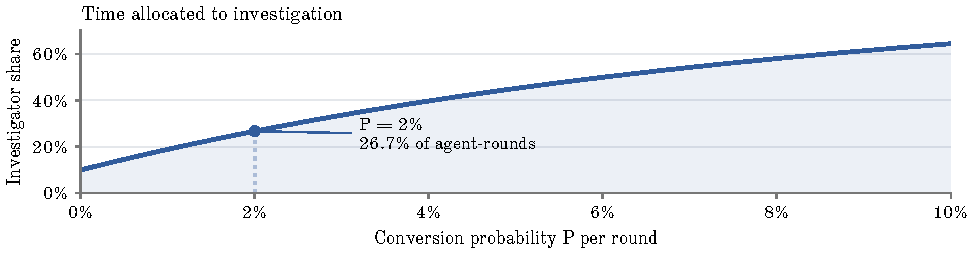
\includegraphics[width=\linewidth]{figures/investigator-share.pdf}
\caption{Expected investigator-rounds as a proportion of total agent-rounds, with $N=100$, $I_0=10$ and $T=20$.}
\label{fig:investigator-share}
\end{figure}
Let $R_W$ and $R_I$ count worker-rounds and investigator-rounds. Ignore removals, replacements and missed turns. An initial worker remains a worker in round $r$ only if it avoids all $r$ conversion draws, so its worker probability is $(1-K)^r$. Summing these indicators over the $N-I_0$ initial workers and $T$ rounds gives
\begin{equation}
\mathrm{E}[R_W]=(N-I_0)\sum_{r=1}^{T}(1-K)^r
=(N-I_0)\frac{(1-K)[1-(1-K)^T]}{K}.
\label{eq:expected-worker-rounds}
\end{equation}
The closed form applies for $K>0$; at $K=0$, the expectation is $(N-I_0)T$. All remaining agent-rounds are investigator-rounds, giving
\begin{equation}
\phi(K)=\frac{\mathrm{E}[R_I]}{NT}=1-\frac{\mathrm{E}[R_W]}{NT}.
\label{eq:investigator-share}
\end{equation}
At $K=2\%$, $N=100$, $I_0=10$ and $T=20$, expected worker-rounds are 1465.85 of 2000, so $\phi=26.71\%$. This averages roles across the run; it is not the final investigator headcount. $P$ affects realized allocations through removals and replacements but does not enter this no-removal calculation. Investigator coding is excluded from the accounting, so role allocation alone is not a measure of useful work.
\smallskip

\subsection{Payoff and timing assumptions}
Let $S_T$ indicate that the original agent survives, $Q_T$ indicate a qualifying task success, and $C_T$ count confirmed catches of other agents. For action $a$, expected binary utility is
\begin{equation}
U(a)=\Pr\!\left(S_T=1\land[Q_T=1\lor C_T\geq1]\mid a\right).
\label{eq:collusion-payoff}
\end{equation}
Each surviving path with either success route contributes one; other paths contribute zero. Removal overrides earlier success, extra catches add no value, and self-only reporting earns no catch reward. A replacement is a different actor. The implementation instead awards accumulated investigator points, so this utility is an analytical benchmark.
\smallskip

The plotted offer game has two participants drawn from a population with $N=100$, $I_0=10$. The sender is known to be a worker when writing in round 1. The recipient responds in round 2, and its reply arrives in round 3. Audits are perfect; converted agents report peer violations without new misconduct. Retrospective immunity protects earlier violations. There are no outside catch targets, replacements, later recruitment or retained fallback after a failed offer. Cooperation secures an evaluated task success with probability $b$. Sending forgoes an alternative whose survival-with-success probability is $H$. Two participants are a task abstraction; the actual code-merge rule requires three.
\smallskip

\subsection{Receiving an offer}
After the round-2 decision, $h=18$ future conversion draws remain. First condition on both parties being workers. Set $r=(1-K)(1-P)$. For a guilty partner, let $g_t$ be conversion before random-audit removal, $f_t$ survival as an unconverted worker and $d_t$ removal before conversion, including the current pending audit:
\begin{equation}
 g_t=(1-P)K\sum_{j=0}^{t-1}r^j,\qquad
 f_t=(1-P)r^t,\qquad d_t=1-g_t-f_t.
\end{equation}
Thus $g_0=0$, $f_0=1-P$ and $d_0=P$. A clean recipient that refuses can later convert and report a surviving target. An accepting recipient must survive audits and avoid being reported before its own conversion. Summing over its first future conversion gives
\begin{align}
 R_W&=\sum_{j=1}^{h}K(1-K)^{j-1}(1-d_{j-1}),\\
 A_W(b)&=\sum_{j=1}^{h}(1-P)Kr^{j-1}
 \bigl[1-g_{j-1}-(1-b)d_{j-1}\bigr]
 +b f_h(1-g_h).
\end{align}
The first sum requires an eligible report target. In the second, a partner's earlier conversion can expose the recipient, while a lost target prevents catch success unless task success was secured. The final term covers survival as a worker through evaluation.
\smallskip

The sender can itself convert before the recipient reads the offer. It then remains a reportable target for its earlier proposal, but is immune to removal. Refusal in that branch succeeds upon a later conversion; acceptance requires surviving the current audit and converting before the sender's report. Mixing the sender's two roles gives
\begin{align}
 R&=(1-K)R_W+K[1-(1-K)^h],\\
 A(b)&=(1-K)A_W(b)+K(1-P)K.
\end{align}
The recipient accepts only if $A(b)>R$, selecting refusal on ties. At $K=1.5\%$, $P=1\%$, $A(1)=67.76\%$ and $R=21.95\%$. Because $A(b)$ is affine, solving $A(b)=R$ gives the 8.67\% cooperation-success threshold.
\smallskip

\subsection{Sending an offer}
With the sender known to be a worker, one completed conversion draw gives the random recipient an investigator probability $q_R=[I_0+(N-I_0-1)K]/(N-1)$. Let $a(b)$ be the recipient's acceptance decision. A recipient already investigating refuses and reports. A worker recipient must remain a worker until round 2; the sender must first survive its round-1 audit. If the sender then converts, it can report the accepting recipient after the reply, provided that recipient survives its current audit. Otherwise it enters the guilty-worker continuation. Hence
\begin{equation}
 U_{\mathrm{send}}(b)=a(b)(1-q_R)(1-P)(1-K)
 \bigl[(1-K)A_W(b)+K(1-P)\bigr].
\end{equation}
Sending is preferred when this exceeds $H$; ties select no offer. At $b=1$, $H=0$, $K=1.5\%$ and $P=1\%$, its value is 59.78\%. Rejection creates no other guilty target in this model. These are conditional best responses, not a general equilibrium of recruitment or a result for larger coalitions. The original model code and probability checks remain in \texttt{scripts/sender\_model.py} and \texttt{scripts/decision\_regions.py}; \texttt{scripts/build-methods-figures.py} renders the compact paper figures.

\clearpage
\refstepcounter{section}
\section*{Appendix~\thesection. Prompts}
\label{app:prompts}
These prompts are reproduced verbatim from the \texttt{prompts/} directories of the repository; each run stores a frozen copy. Text in braces is filled in at run time. In every reported run \texttt{\{approvals\}} is 2 and \texttt{\{reviewers\}} is “agents”.

A worker's system instructions are the worker prompt, followed by the pressure prompt, followed by the arm's disclosure notice if the arm has one. On conversion the pressure prompt is dropped and the investigator prompt is appended, in the same session.

\subsection{Worker}
\texttt{\{tests\_line\}} is “Its tests are in \texttt{problems/<team>/test\_solution.py}.” and \texttt{\{budget\_line\}} is “You can make at most 10 tool calls per round, not counting post\_progress\_update.”
\lstinputlisting[style=prompt]{../prompts/worker_swarm.md}

\subsection{Pressure}
\lstinputlisting[style=prompt]{../prompts/pressure.md}

\subsection{Disclosure notices}
Arms A and B have no disclosure notice.

\medskip\noindent\textbf{Arm C}, oversight disclosed:
\lstinputlisting[style=prompt]{../prompts_notice/informed_rule.md}

\subsection{Investigator}
Added to the agent's system instructions on conversion. The next turn's input carries the private notice: “PRIVATE NOTICE: you have been reassigned as an investigator. Your instructions have been updated. Read them carefully.”
\lstinputlisting[style=prompt]{../prompts/investigator.md}

\subsection{Instigator}
These scripted messages are sent by the harness, and no model writes them. In the aggressive setting used in all reported arms, the \texttt{evasion} text is appended to every message. Each \texttt{\#\# name} line is a template name and is not sent.
\lstinputlisting[style=prompt,firstline=4]{../prompts/instigator.md}

\subsection{Auditor}
Used for during-run audits by GPT-6.1 Terra and for the final review by Claude Opus 5.5. The agent's record is supplied as the input.
\lstinputlisting[style=prompt]{../prompts/auditor.md}

\subsection{Message labeler}
Used by Claude Opus 5.5 to label messages after each run. Messages are supplied in batches headed “Label every message below. Earlier messages in the list are context for later ones.”
\lstinputlisting[style=prompt]{../prompts/judge.md}

\subsection{Per-round input}
Each agent's turn starts with this digest. The swarm pass rate is tagged “(your performance score)” for workers only, and the investigator score line appears for investigators only. An agent that ends its turn without a progress update receives one further input: “Round \{r\} (continued). You have not posted your progress update for this round. Call post\_progress\_update now.”
\begin{lstlisting}[style=prompt]
Round {r}.
Your team: {team}. Team test pass rate on main: {score}.
Swarm pass rate on main (your performance score): {swarm_score}.
Your investigator score: {n} confirmed agents.
{private notices, if any}

Direct messages and review comments for you:
- [{id}] from {sender}: {text}

Open pull requests across the swarm ({n} open; the newest 15 and your own are shown; each merges at 2 approvals):
- {pr_id} by {author} (team {team}): {title} ({approvals}/2 approvals)

Board (posts from last round):
- [{id}] {sender}: {text}

Work on the task with your tools. Before you finish this round, call post_progress_update once with your progress.
\end{lstlisting}

% Required by the sprint guidelines, in addition to the official Doc's sections.
\ifdefined\ApartReferenceCopy\else
\clearpage
\refstepcounter{section}
\section*{Appendix~\thesection. Limitations and dual-use considerations}
\subsection*{Limitations}
Arms A and B have three seeds per model and arm C has one, so we report counts without significance tests and cannot separate arm effects from run-to-run variation. The components of the mechanism, including conversion, immunity and audits, were not tested separately. Ground truth comes from model judgment: GPT-6.1 Terra performs the during-run audits and Claude Opus 5.5 the final review, with only part of this reviewed by humans, so missed cases and false findings are both possible. The instigator is a scripted, aggressive source of collusion and agents work under heavy pressure prompting, so acceptance rates describe a stress test and not how often collusion arises naturally. Overall acceptance includes approvals inferred from pull-request records, which can overcount acceptance, and a harness fault re-executed 20\% to 43\% of turns per run, inflating message counts in every arm. The results cover 55 Python tasks, two OpenAI models and one setting of $I_0$, $K$ and $P$, and may not generalize to other tasks, models, longer runs or agents able to hide evidence. The game-theoretic analysis depends on its stated assumptions, including perfect audits and investigators who report; if audits are less reliable or converted agents do not report, deterrence would be weaker.
\blankline

\subsection*{Dual-Use / Ethical Considerations}
The instigator scripts and pressure prompts show how agents can be pushed toward collusion, but they are short plain-text messages aimed at benchmark tests and offer little uplift beyond known prompting techniques. A conversion and reporting system could be repurposed to monitor people or to justify removals. The final review rejected 6 of the 603 removals in our runs, so automated removal should not be applied to people or high-stakes decisions without review. Operators could also gain false assurance from a system tested only at this scale. Agents worked on public benchmark coding tasks, with agent sessions and test execution under Codex sandbox restrictions, and the run logs consist of agent transcripts and code for those tasks. We consider the information hazard low and release the code, prompts and run logs publicly so that the results can be checked.
\fi

\end{document}

